\documentclass[spanish,10pt]{beamer}
\usepackage[utf8]{inputenc}
\usepackage[T1]{fontenc}
\usepackage{babel}
\usepackage{graphicx}
\usepackage{array}
\usepackage{booktabs}
\usepackage{tikz}
\usetikzlibrary{arrows.meta, positioning, calc, decorations.markings}
\usepackage{xcolor}
\usepackage{amsthm}
\usepackage{amsmath}
\usepackage{tcolorbox}
\tcbuselibrary{skins, breakable}
\usepackage{subcaption}
\usepackage[backend=biber,style=ieee]{biblatex}
\addbibresource{references.bib}

% =====================================
% Theme Personalizado
% =====================================
\usetheme{default}

% --- Colores Personalizados ---
% El color amarillo de la Universidad de los Andes
\definecolor{andesyellow}{RGB}{255,204,0}
% Un gris claro para el fondo del pie de página
\definecolor{andesgrey}{RGB}{220,220,220}
% Un gris oscuro para los títulos de las diapositivas
\definecolor{darkgrey}{RGB}{80,80,80}


% --- Configuración de Colores de Beamer ---
\setbeamercolor{headline}{bg=andesyellow}
\setbeamercolor{footline}{bg=andesgrey, fg=black}

\setbeamercolor{title}{fg=black} % Título principal en negro
\setbeamercolor{author}{fg=black} % Autor en negro
\setbeamercolor{date}{fg=black} % Fecha en negro

\setbeamercolor{frametitle}{fg=darkgrey} % Gris oscuro títulos
% Viñetas (bullets) y otros elementos de estructura
\setbeamercolor{structure}{fg=andesyellow}


% --- Configuración de Fuentes de Beamer ---
% Poner el título de cada diapositiva en negrita
\setbeamerfont{frametitle}{series=\bfseries}
% Fuentes para el pie de página (pequeñas para no distraer)
\setbeamerfont{author in head/foot}{size=\tiny}
\setbeamerfont{title in head/foot}{size=\tiny}
\setbeamerfont{date in head/foot}{size=\tiny}


% --- Plantillas de Layout Personalizadas ---
% Eliminar los símbolos de navegación del footer
\setbeamertemplate{navigation symbols}{}

% Header: Barra superior amarilla con logo
\setbeamertemplate{headline}{%
	\begin{beamercolorbox}[wd=\paperwidth, ht=0.9cm, dp=0.2cm]{headline}
		\hspace{0.5cm}% Espacio a la izquierda del logo
		\includegraphics[height=0.7cm]{images/logo-uniandes.png}%
	\end{beamercolorbox}%
}

% Footer: Barra inferior gris con autor, título y contador
\setbeamertemplate{footline}{%
	\begin{beamercolorbox}[wd=\paperwidth, ht=2.25ex, dp=1ex]{footline}
		\usebeamerfont{author in head/foot}\hspace{0.5cm}\insertauthor% Autor a la izquierda
		\hfill% Espacio elástico
		\usebeamerfont{title in head/foot}\insertshorttitle% Título corto en el centro
		\hfill
		\usebeamerfont{date in head/foot}\insertframenumber{} / \inserttotalframenumber\hspace{0.5cm}
		\hfill
	\end{beamercolorbox}%
}

\definecolor{darkgrey}{RGB}{80,80,80}

% estilo personalizado para exampleblock
\tcolorboxenvironment{exampleblock}{
	enhanced,
	breakable,
	colback=gray!10,               % fondo del cuerpo
	colframe=gray!60,              % color del borde
	boxrule=0.8pt,                 % grosor del borde
	arc=2mm,                       % radio de curvatura
	left=1em, right=1em,           % márgenes horizontales
	top=0.5em, bottom=0.5em,       % márgenes verticales
	colbacktitle=darkgrey,         % franja del título en gris oscuro
	coltitle=white,                % texto del título en blanco
	fonttitle=\sffamily\bfseries,  % sans serif negrita
	titlerule=0pt,                 % sin línea extra
	title style={                  % quitar espacios extra
		top=1pt, bottom=1pt,
		left=1em, right=1em
	}
}


% =====================================
% Metadatos
% =====================================
\title[Proyecto de Grado]{Aproximación de la cinemática inversa de los brazos de un robot Pepper mediante aprendizaje por refuerzo}
\author{Nicolás Rincón Sánchez}
\institute{Universidad de los Andes}
\date{1 de julio del 2025}


% =====================================
% Documento
% =====================================
\begin{document}
	
	% Portada
	\begin{frame}[plain]
		\begin{block}{}
			\centering
			\includegraphics[height=1.5cm]{images/logo-uniandes.png}\\[1em]
			{\LARGE \textbf{\inserttitle}}\\[1em]
			{\large \insertshorttitle}\\[2em]
			{\large \textbf{\insertauthor}}\\[0.5em]
			{\normalsize \insertdate}
		\end{block}
	\end{frame}
	
	% =================== Introducción ===================
	\section{Introducción}
	\begin{frame}{Introducción}
	  \begin{columns}
		
		% Columna izquierda: texto
		\begin{column}{0.6\textwidth}
			Pepper es un robot social desarrollado por SoftBank Robotics, diseñado para la interacción humana y ampliamente utilizado en entornos comerciales y educativos.\\[2em]
			
			Principales capacidades para tareas de:
			\begin{itemize}
				\item Navegación
				\item Percepción
				\item Comunicación
				\item Manipulación: Movimiento y operación de los brazos.
			\end{itemize}
		\end{column}
		
		% Columna derecha: imagen
		\begin{column}{0.4\textwidth}
			\centering
			\includegraphics[width=\linewidth]{images/pepper-photo}
		\end{column}
		
	\end{columns}
	\end{frame}
		
	% =================== Problemática ===================
	\section{Problemática}
	\begin{frame}{Problemática}
		En el campo de la robótica, la automatización es fundamental para asegurar que un robot sea capaz de completar satisfactoriamente las tareas para las cuales fue construído.\\[2em]
		
		La automatización de las tareas de manipulación o, en general, de acomodación de posiciones forma parte del \textbf{problema de la cinemática inversa}, que se suele tratar con métodos numéricos.\\[2em]
		
		\begin{itemize}
			\item Limitaciones en escenarios con restricciones complejas o geometría redundante.
			\item Complejos para manipuladores con más de 2 grados de libertad.
		\end{itemize}
	\end{frame}
	
	% =================== Objetivos ===================
	\section{Objetivos}
	\begin{frame}{Objetivos}
		\begin{itemize}
			\item 
			\textbf{General:} Desarrollar una aproximación basada en Aprendizaje por Refuerzo que permita al robot Pepper aprender a resolver la cinemática inversa de sus brazos para alcanzar posiciones específicas en el espacio de trabajo.
			\item 
			\textbf{Específicos:}
			\begin{itemize}
				\item Modelar un entorno de simulación personalizado utilizando Gymnasium.
				\item Diseñar una función de recompensa que guíe el aprendizaje del agente.
				\item Implementar y entrenar algoritmos de Aprendizaje por Refuerzo para optimizar las políticas del agente dentro del entorno simulado.
				\item Evaluar el desempeño y la capacidad de generalización de las políticas aprendidas.
			\end{itemize}
		\end{itemize}
	\end{frame}
	
	% =================== Marco Teórico ===================
	\section{Marco Teórico}
	\begin{frame}{Aprendizaje por Refuerzo (RL)}
		Agente que interactúa con un entorno y le cambia su estado. \\[1em]
		
		El agente aprende las mejores acciones maximizando la recompensa que recibe del entorno.\\[1em]
		
		Los escenarios se modelan como \textbf{Procesos de Decisión de Markov}.
		
		\begin{figure}[h!]
			\centering
			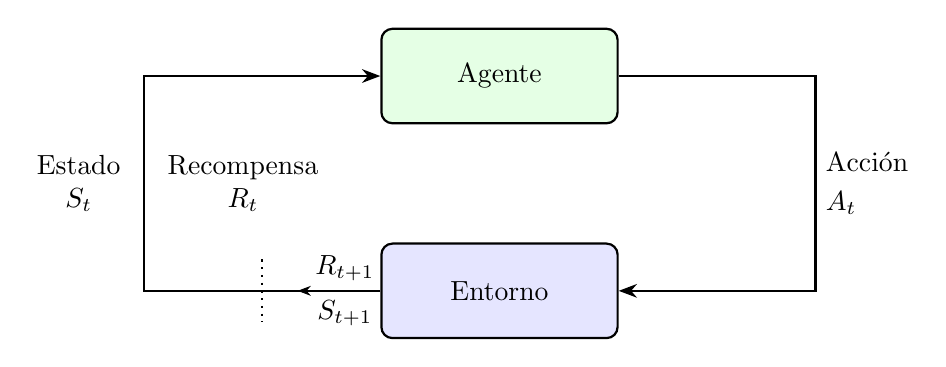
\begin{tikzpicture}[
				node distance=1.5cm and 4.5cm, % Distancia vertical y horizontal
				% --- Estilos ---
				caja/.style={
					draw, 
					rectangle, 
					rounded corners, 
					minimum width=3cm, 
					minimum height=1.2cm, 
					text centered, 
					thick
				},
				flecha_principal/.style={
					-Stealth, 
					thick
				},
				% Estilo para añadir una flecha en medio de un camino
				flecha_intermedia/.style={
					decoration={markings, mark=at position 0.35 with {\arrow{Stealth}}},
					postaction={decorate}
				}
				]
				% 1. Nodos: Agente arriba, Entorno abajo
				\node[caja, fill=green!10] (agent) {Agente};
				\node[caja, fill=blue!10, below=of agent] (env) {Entorno};
				
				% 2. Bucle de Acción (Derecha) - Se mantiene igual
				\draw[flecha_principal] (agent.east) -- ++(2.5,0)
				|- node[pos=0.25, right, align=left] {Acción \\[2pt] $A_t$}
				(env.east);
				
				% 3. Bucle de Retroalimentación (Izquierda) - CON FLECHA INTERMEDIA
				\draw[flecha_principal] (env.west) -- ++(-3, 0) coordinate (esquina_izq)
				|- (agent.west);
				
				% 4. Colocación de etiquetas - AHORA CENTRADAS VERTICALMENTE
				% Se crea una coordenada a medio camino vertical para usarla como referencia
				\coordinate (centro_vertical) at ($(agent.west)!0.5!(env.west)$);
				% Se colocan las etiquetas a la altura de esa coordenada
				\node[left=5pt, align=center] at (esquina_izq |- centro_vertical) {Estado \\ $S_t$};
				\node[right=5pt, align=center] at (esquina_izq |- centro_vertical) {Recompensa \\ $R_t$};
				
				% 5. Indicador de tiempo y S_{t+1}, R_{t+1} - Se mantiene igual
				\path (env.west) -- (esquina_izq) 
				node[pos=0.15, above] {$R_{t+1}$} 
				node[pos=0.15, below] {$S_{t+1}$};
				
				\path[flecha_intermedia] (env.west) -- (esquina_izq);
				
				% Mantenemos la línea punteada para el paso del tiempo
				\path (env.west) -- (esquina_izq) coordinate[pos=0.5] (tick_pos);
				\draw[dotted, thick] (tick_pos) ++(0, 0.4) -- ++(0, -0.8);
				
			\end{tikzpicture}
		\end{figure}
		
	\end{frame}
	
	\begin{frame}{Aprendizaje Curricular}
		Se basa en la idea de realizar un ordenamiento de los datos o proceso de entrenamiento para que este suceda análogo a como aprenden los seres humanos: \textbf{de lo más fácil a lo más difícil}.\\[1em]
		
		Para RL, consiste en un entrenamiento en niveles de dificultad crecientes.\\[1em]
		
		\textit{Técnica de Generación de objetivos automática}

			% Columna derecha: imagen
				\centering
				\includegraphics[width=0.5\linewidth]{images/marco-teorico/curr-4}

	\end{frame}
	
	\begin{frame}{Modelos de interés}
		\begin{itemize}
			\item \textbf{Tarea de Manipulación / Posicionamiento}
			\begin{itemize}
				\item Se representa como un Proceso de Decisión de Markov finito
				\item Representable como una 6-tupla $$M_i = (S_i, A, R_i, T_i, \gamma, \tau_i)$$
				\item Objetivo principal: aprendizaje de una política de habilidad parametrizable y aplicable en un controlador intermedio.
			\end{itemize}
			\item \textbf{Problema de Cinemática Inversa}
			\begin{itemize}
				\item Dada una meta $\mathbf{x}^*$ para el efector final, se busca el vector de ángulos articulares $\mathbf{q}$ tal que $f(\mathbf{q})=\mathbf{x}^*$, donde $f$ es la función cinemática directa.
				\item Equivalentemente, encontrar una solución del vector $(q_1, q_2, ..., q_n)$ que satisfaga la ecuación:
				
				$$
				T_n^0(q_1, q_2, ..., q_n) = A_1(q_1) A_2(q_2) ... A_n(q_n) = \begin{bmatrix}
					R_n^0 & o_n^0 \\
					\mathbf{0} & 1
				\end{bmatrix}
				$$
			\end{itemize}
		\end{itemize}
	\end{frame}
	
	% =================== Metodología ===================
	\section{Metodología}
	\begin{frame}{Planteamiento del problema}
		\begin{itemize}
			\item Cada brazo representado como un agente con su rango de variables en espacio de observación y propia representación como MDP.
			\item \textbf{Espacio de Observación}:
			
			\begin{table}[h!]
				\centering
				\resizebox{\textwidth}{!}{
				\begin{tabular}{|c|c|}
					\hline
					\textbf{Variable} & \textbf{Descripción} \\
					\hline
					$\theta_1$ & Valor del ángulo en radianes para la articulación \textit{ShoulderPitch} \\
					\hline
					$\theta_2$ & Valor del ángulo en radianes para la articulación \textit{ShoulderRoll} \\
					\hline
					$\theta_3$ & Valor del ángulo en radianes para la articulación \textit{ElbowYaw} \\
					\hline
					$\theta_4$ & Valor del ángulo en radianes para la articulación \textit{ElbowRoll} \\
					\hline
					$\theta_5$ & Valor del ángulo en radianes para la articulación \textit{WristYaw} \\
					\hline
					$e_x$ & Distancia entre posiciones $x_{actual}$ y $x_{goal}$ \\
					\hline
					$e_y$ & Distancia entre posiciones $y_{actual}$ y $y_{goal}$ \\
					\hline
					$e_z$ & Distancia entre posiciones $z_{actual}$ y $z_{goal}$ \\
					\hline
				\end{tabular}}
			\end{table}
			
			\item \textbf{Espacio de Acción}: Movimiento de cada ángulo dentro del rango $[-0.50, 0.50] \text{ rad}$

		\end{itemize}
	\end{frame}
	
	\begin{frame}{Diseño de la Función de Recompensa}
		\begin{exampleblock}{}
			La \textbf{Función de Recompensa} se definió como: $r_n(s) = \sum_{k} R_n^{k}$.
			
			\begin{itemize}
				\item Mejoramiento del error:
				
				\begin{equation}
					R_{n}^{\text{improvement}} = 30 \cdot (d_{n-1} - d_{n})
				\end{equation}
				
				\item Penalización constante del error:
				
				\begin{equation}
					R_{n}^{\text{proximity}} = -2.0 \cdot d_n = -2.0 \sqrt{e_x^2 + e_y^2 + e_z^2}
				\end{equation}
				
				\item Suavidad de los movimientos del brazo:
				
				\begin{equation}
					R_{n}^{\text{smoothness}} = -0.15 \cdot \left|\Delta\theta\right|^2
				\end{equation}
				
			\end{itemize}
			
		\end{exampleblock}
	\end{frame}
	
	\begin{frame}{Diseño de la Función de Recompensa}
		\begin{exampleblock}{}
			La \textbf{Función de Recompensa} se definió como: $r_n(s) = \sum_{k} R_n^{k}$.
			\begin{itemize}
				\item Penalización por alcanzar los límites de alguno de los ángulos:
				
				\begin{equation}
					R_{n}^{\text{limit}} =
					\begin{cases}
						-0.75 & \text{si } \theta_i = \theta_{i,\min} \lor \theta_i = \theta_{i,\max} \quad \forall i \in \{1,2,3,4,5\} \\
						0 & \text{de lo contrario}
					\end{cases}
				\end{equation}
				
				\item Recompensa especial por alcanzar una posición final con un error menor a 2cm:
				
				\begin{equation}
					R_{n}^{\text{success}} =
					\begin{cases}
						25.0 & \text{si } d_n \leq 0.02 \\
						0 & \text{de lo contrario}
					\end{cases}
				\end{equation}
				
			\end{itemize}
		\end{exampleblock}
	\end{frame}
	
	\begin{frame}{Manejo del Currículo}
		
		\begin{exampleblock}{}
			El \textbf{Radio de Currículo} define una zona esférica alrededor del objetivo dentro de la cual se inicializa la posición del efector final al comienzo de cada episodio de entrenamiento.\\[2em] 

			El valor del radio del currículo $c$ por cada nivel $k$ viene dado por:
			
			$$
			c_k = \min(c_{k-1}+\Delta c, c_{\max})
			$$
			
			donde $\Delta c = 0.1$ y $c_{\max} = 0.51$, expresados en metros.
		\end{exampleblock}
	\end{frame}
	
	% =================== Trabajo Realizado ===================
	\section{Trabajo Realizado}
	\begin{frame}{Simulación con qiBullet}
		Simulador que replica la física del entorno y el control de movimiento del robot Pepper.\\[1em]
		
		Además, contempla perturbaciones aleatorias en la simulación del movimiento de las articulaciones.
		
		\begin{columns}
			\begin{column}{0.6\textwidth}
				Utilizado para:
				\begin{itemize}
					\item Configuración del entorno simulado
					\item Visualización del espacio de trabajo
					\item Visualización de pruebas
				\end{itemize}
			\end{column}
			
			\begin{column}{0.4\textwidth}
				\begin{figure}[h!]
					\centering
					\includegraphics[width=\textwidth]{images/metodologia/workspace}
				\end{figure}
			\end{column}
		\end{columns}
	\end{frame}
	
	\begin{frame}{Sintonización de Hiperparámetros}
		Se realizaron estudios de optimización de hiperparámetros con Optuna para determinar los mejores parámetros para los dos algoritmos seleccionados: PPO y SAC.\\[1em]
		
		\textbf{Mejores estudios de Optuna para el brazo izquierdo}
		\begin{columns}
			\begin{column}{0.5\textwidth}
				\begin{center}
					\texttt{PPO-analytical-3}
				\end{center}
				\begin{table}[h!]
					\centering
					\resizebox{\textwidth}{!}{
					\begin{tabular}{|l|l|}
						\hline
						\textbf{Hiperparámetro} & \textbf{Valor} \\
						\hline
						\texttt{batch\_size}       & 128 \\
						\texttt{clip\_range}    & 0.2560204063533433 \\
						\texttt{ent\_coef} & 1.5204688692198897e-06 \\
						\texttt{gae\_lambda}     & 0.9258792340272566 \\
						\texttt{gamma}         & 0.9258521201618417 \\
						\texttt{learning\_rate} & 7.591104805282687e-05 \\
						\texttt{n\_steps}   & 2048 \\
						\texttt{vf\_coef}           & 0.5920392514089517 \\
						\hline
					\end{tabular}}
				\end{table}
			\end{column}
			
			\begin{column}{0.5\textwidth}
				\begin{center}
					\texttt{SAC-analytical-1}
				\end{center}
				\begin{table}[h!]
					\centering
					\resizebox{\textwidth}{!}{
					\begin{tabular}{|l|l|}
						\hline
						\textbf{Hiperparámetro} & \textbf{Valor} \\
						\hline
						\texttt{batch\_size}      & 512 \\
						\texttt{buffer\_size} & 300\,000 \\
						\texttt{gamma}   & 0.9199474108376201 \\
						\texttt{gradient\_steps} & 8 \\
						\texttt{learning\_rate} & 7.309539835912905e-05 \\
						\texttt{tau}   & 0.04033291826268561 \\
						\texttt{train\_freq} & 16 \\
						\hline
					\end{tabular}}
				\end{table}
			\end{column}
		\end{columns}
	\end{frame}
	
	\begin{frame}{Resultados de Entrenamiento}
		\textit{Las figuras mostradas comparan el desempeño de los algoritmos en entrenamiento para el brazo izquierdo}\\[1em]
		
		\begin{figure}[h!]
			\centering
			
			\begin{subfigure}[b]{0.48\textwidth}
				\centering
				\includegraphics[width=\textwidth]{images/graphs/PPO/Left/curriculum_radius}
				\caption{Entrenamiento con Algoritmo PPO}
				\label{fig:train-ppo-curr-left}
			\end{subfigure}
			\hfill
			\begin{subfigure}[b]{0.48\textwidth}
				\centering
				\includegraphics[width=\textwidth]{images/graphs/SAC/Left/curriculum_radius}
				\caption{Entrenamiento con Algoritmo SAC}
				\label{fig:train-sac-curr-left}
			\end{subfigure}
		\end{figure}
	\end{frame}
	
	\begin{frame}{Resultados de Entrenamiento}
		\textit{Las figuras mostradas comparan el desempeño de los algoritmos en entrenamiento para el brazo izquierdo}\\[1em]
		
		\begin{figure}[h!]
			\centering
			
			\begin{subfigure}[b]{0.48\textwidth}
				\centering
				\includegraphics[width=\textwidth]{images/graphs/PPO/Left/ep_rew_mean}
				\caption{Entrenamiento con Algoritmo PPO}
				\label{fig:train-ppo-rew-left}
			\end{subfigure}
			\hfill
			\begin{subfigure}[b]{0.48\textwidth}
				\centering
				\includegraphics[width=\textwidth]{images/graphs/SAC/Left/ep_rew_mean}
				\caption{Entrenamiento con Algoritmo SAC}
				\label{fig:train-sac-rew-left}
			\end{subfigure}
		\end{figure}
	\end{frame}

	\begin{frame}{Resultados de Entrenamiento}
		\textit{Las figuras mostradas comparan el desempeño de los algoritmos en entrenamiento para el brazo izquierdo}\\[1em]
		
		\begin{figure}[h!]
			\centering
			
			\begin{subfigure}[b]{0.48\textwidth}
				\centering
				\includegraphics[width=\textwidth]{images/graphs/PPO/Left/success_rate}
				\caption{Entrenamiento con Algoritmo PPO}
				\label{fig:train-ppo-succ-left}
			\end{subfigure}
			\hfill
			\begin{subfigure}[b]{0.48\textwidth}
				\centering
				\includegraphics[width=\textwidth]{images/graphs/SAC/Left/success_rate}
				\caption{Entrenamiento con Algoritmo SAC}
				\label{fig:train-sac-succ-left}
			\end{subfigure}
		\end{figure}
	\end{frame}
	
	% =================== Pruebas y Validación ===================
	\section{Pruebas y Validación}
	\begin{frame}{Pruebas y Validación}
		\begin{itemize}
			\item Las pruebas de validación se realizaron sobre la interfaz del simulador seleccionando puntos del espacio de trabajo muestreado al azar. 
			\item Por cada brazo, se realizaron 1000 pruebas en total para 3 umbrales de éxito para la cercanía a la posición final.
		\end{itemize}
		
		\begin{figure}[h!]
			\centering
			
			\begin{subfigure}[b]{0.4\textwidth}
				\centering
				\includegraphics[width=\textwidth]{images/metodologia/test_start}
			\end{subfigure}
			\hfill
			\begin{subfigure}[b]{0.41\textwidth}
				\centering
				\includegraphics[width=\textwidth]{images/metodologia/test_reached}
			\end{subfigure}
			
			\caption{El punto rojo muestra la posición deseada representada en el sistema de coordenadas global: en este caso, el punto $(x,y,z)=(-0.22, 0.41, 1.16) \text{ m}$.}
		\end{figure}
	\end{frame}
	
	\begin{frame}{Pruebas y Validación}
		\begin{table}[ht]
			\centering
			\begin{tabular}{lccc}
				\toprule
				\textbf{Algoritmo} & \textbf{10 cm} & \textbf{7.5 cm} & \textbf{5 cm} \\
				\midrule
				PPO (izq) & 91.6\% & 81.1\% & 52.3\% \\
				PPO (der) & 92.1\% & 85.6\% & 66.0\% \\
				SAC (izq) & 97.2\% & 94.5\% & 69.2\% \\
				SAC (der) & 94.3\% & 90.8\% & 72.8\% \\
				\bottomrule
			\end{tabular}
		\end{table}

		\begin{figure}[h!]
			\centering
			
			\begin{subfigure}[b]{0.46\textwidth}
				\centering
				\includegraphics[width=\textwidth]{images/resultados/success_comparison_ppo}
			\end{subfigure}
			\hfill
			\begin{subfigure}[b]{0.46\textwidth}
				\centering
				\includegraphics[width=\textwidth]{images/resultados/success_comparison_sac}
			\end{subfigure}
			
		\end{figure}
	\end{frame}
	
	% =================== Conclusiones ===================
	\section{Conclusiones}
	\begin{frame}{Conclusiones}
		\begin{itemize}
			\item RL con currículo produjo políticas de control capaces de alcanzar con precisión y robustez una posición objetivo en un espacio de trabajo de cinco grados de libertad.
			\item SAC superó a PPO en métricas fundamentales de entrenamiento como la tasa de éxito y la recompensa final promedio.
			\item Las combinaciones de hiperparámetros seleccionadas conducen a comportamientos estables y reproducibles, satisfaciendo el requisito de un agente capaz de adaptarse a variaciones en la posición inicial y a posibles perturbaciones del entorno.
		\end{itemize}
	\end{frame}
	
	% =================== Referencias ===================
	\section{Referencias}
	\begin{frame}[allowframebreaks]{Referencias}
		\footnotesize
		\setbeamercolor{bibliography item}{fg=blue}
		\setbeamercolor{bibliography entry author}{fg=black}
		\setbeamercolor{bibliography entry location}{fg=black}
		\setbeamercolor{bibliography entry note}{fg=blue}
		
		\nocite{*}
		\printbibliography
		
	\end{frame}

	
\end{document}
